
\section{Critical densities and phase diagrams}
\begin{frame}{$d_u^\theta$ measures directions that are difficult to infect}
	\begin{block}{Critical densities with conic boundary conditions}
		For $u\in \mathbb{S}^1$ and $\theta\in[-\pi, \pi]$
		$$d_u^\theta := \inf\left\{q\in[0,1], \sum_n n\mathbb{P}_q(0\not\in [(A\cup V_{u,u+\theta})\cap B_n]) < \infty\right\}$$
	\end{block}
	Morally, the critical probability with infection of $V_{u,u+\theta} = \mathbb{H}_u \cap \mathbb{H}_{u+\theta}$. 
	\begin{itemize}
		\item The summand decays slowly in $n$ when it is hard to infect the origin using only infections at distance less than $n$. So, when it is hard to infect 0,  $d_u^\theta$ is large\footnote{non zero...}.
		\item When $\theta \sim \pm \pi$, few sites are infected, so it is easy for the origin not to be infected, the summand can be large. Hence, $d_u^\theta$ decreases when $\theta\to 0$.
	\end{itemize}
\end{frame}




\begin{frame}

	\begin{theorem}
		For any $\mathcal{U}$-bootstrap percolation model, its critical probability
		\begin{equation*}
			\tilde q_c = \inf\{q\in[0,1], \sum_n n\mathbb{P}_q(0\not\in [A\cap B_n]) < \infty\}
		\end{equation*}
		is equal to the maximal value of its critical density function
		\begin{equation*}
			d_u = \max_{0^\pm} \inf\{q\in[0,1], \sum_n n\mathbb{P}_q(0\not\in[(A\cup V_{u, u + 0^\pm})\cap B_n] < \infty\}
		\end{equation*}
		for $u$ in any semicircle $C$, i.e.,
		\begin{equation*}
			\tilde q_c = \inf_{C\in \mathcal{C}} \sup_{u\in C} d_u.
		\end{equation*}

	\end{theorem}

\end{frame}

\begin{frame}{Phase diagram in a fixed direction $u$}
	\begin{center}
    	 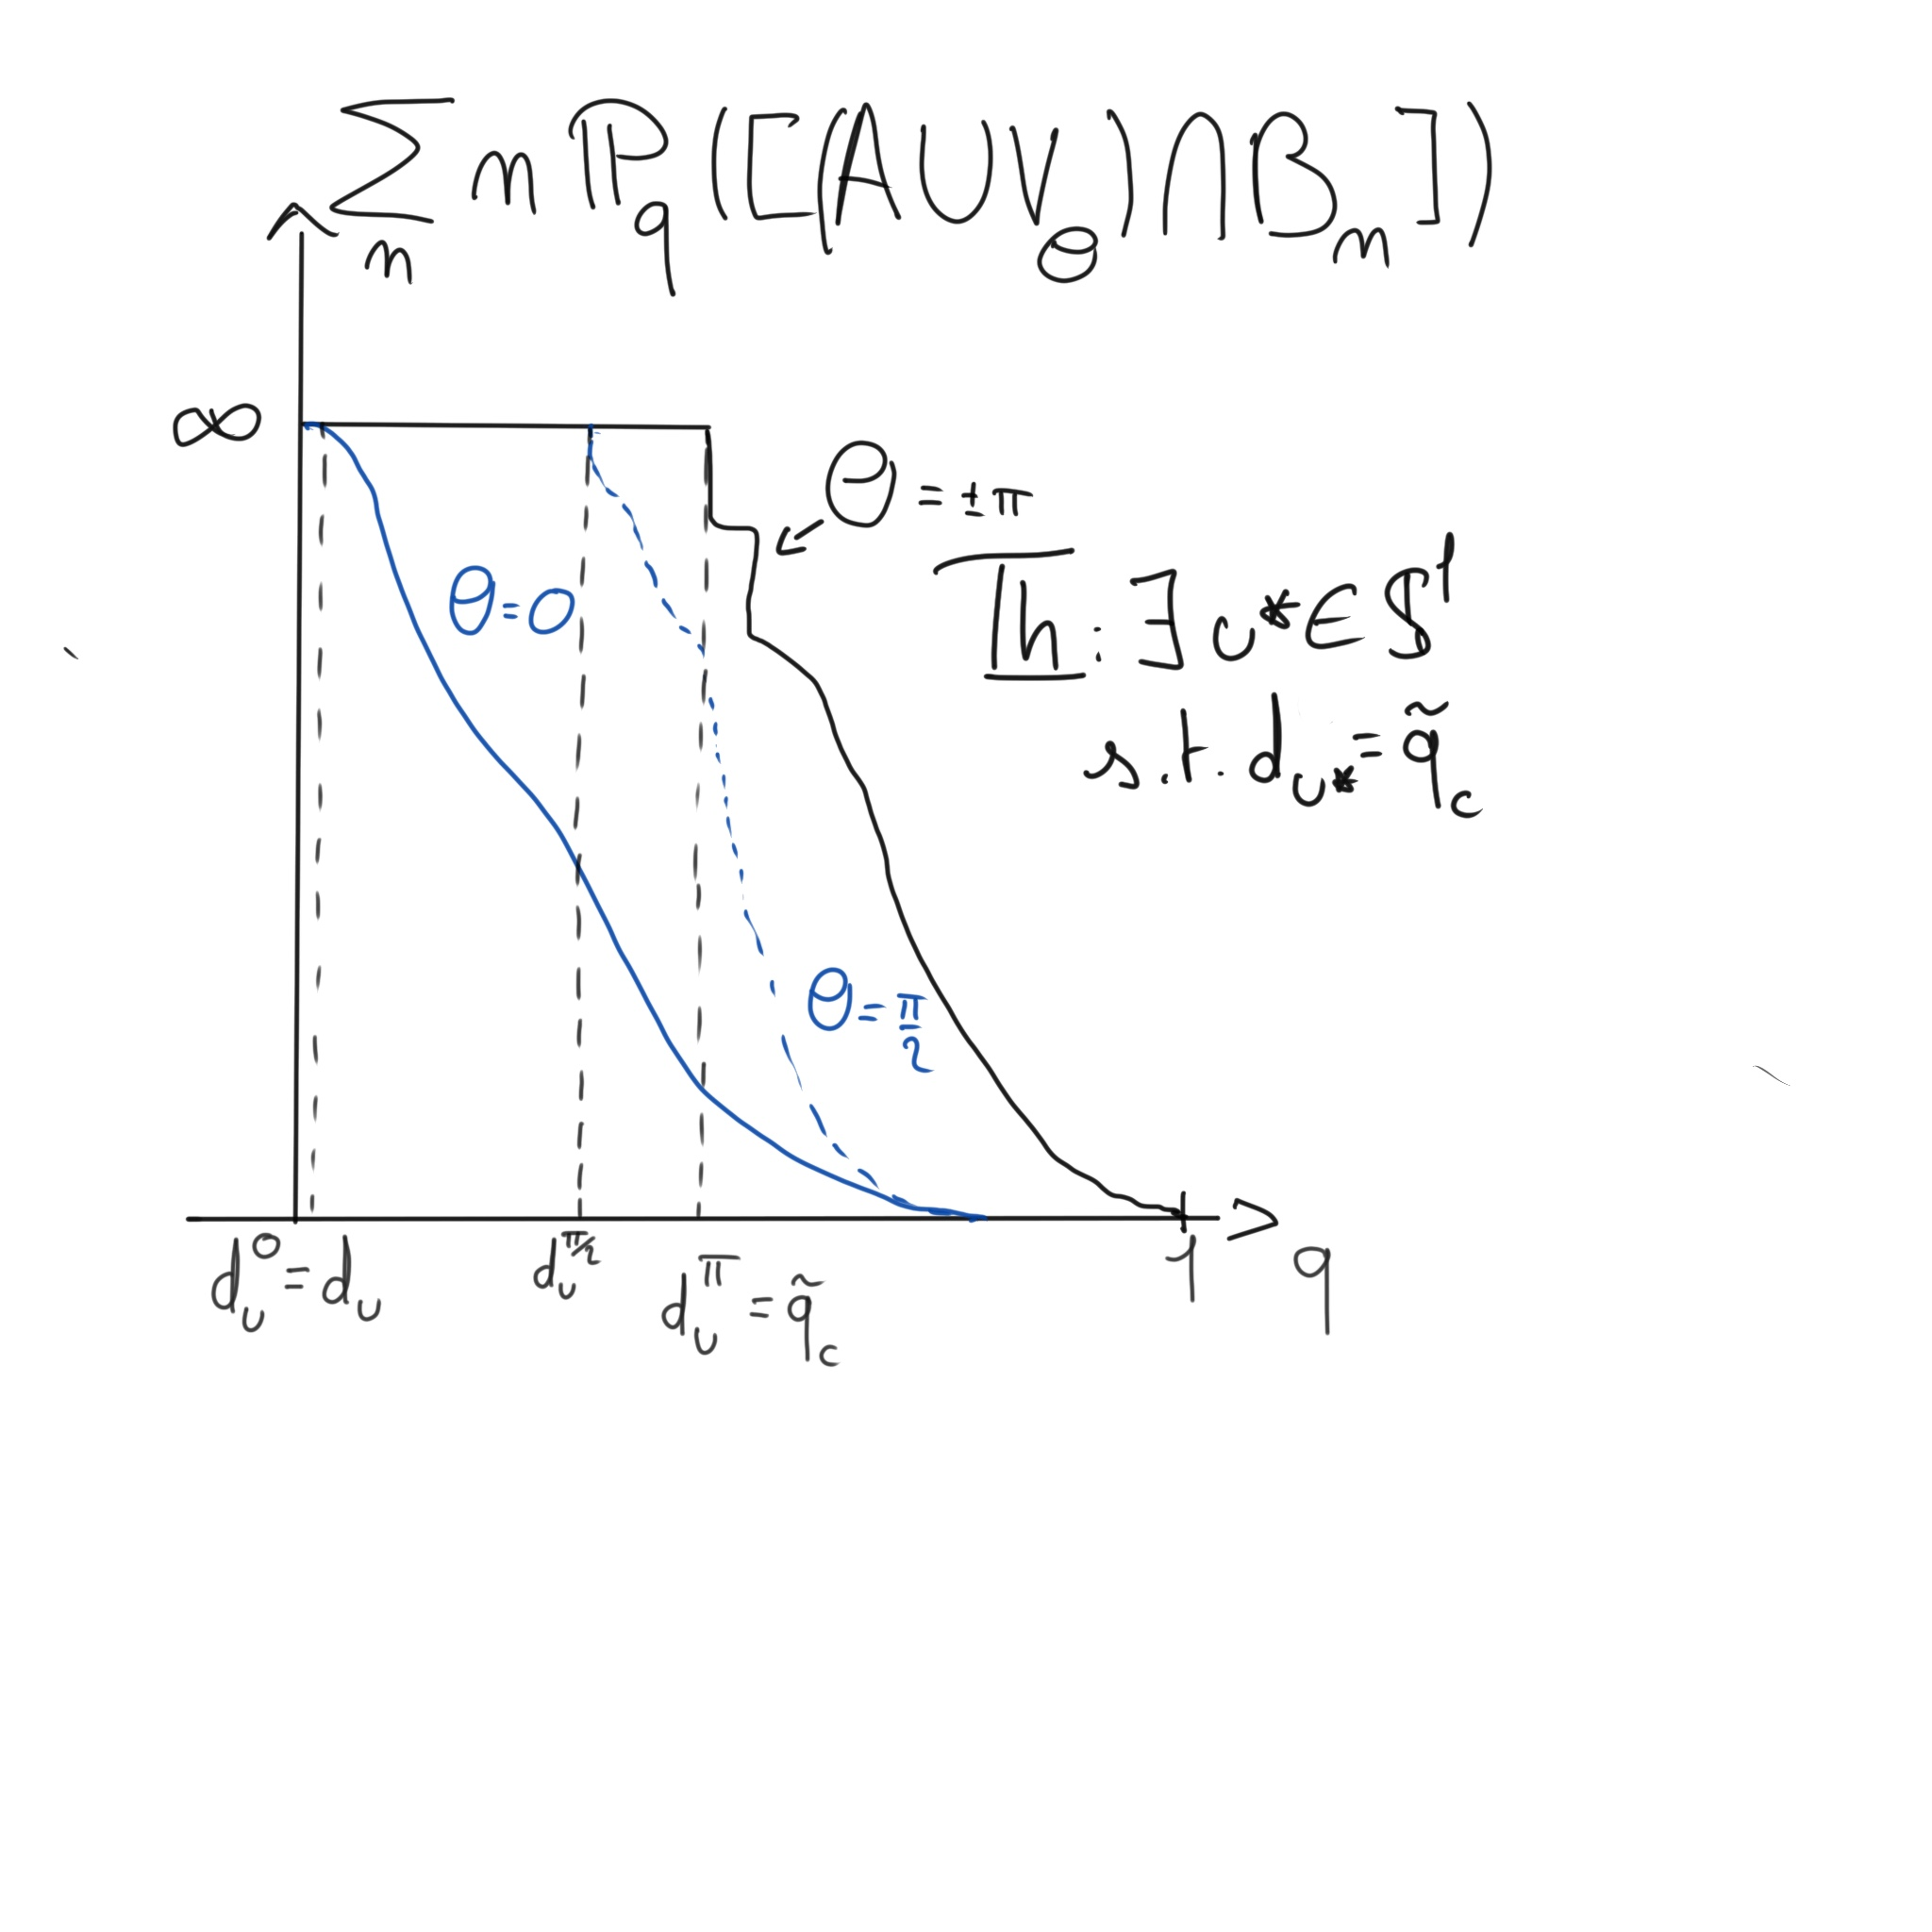
\includegraphics[width=\textwidth]{decay_theta.jpg}
	\end{center}

\end{frame}

\begin{frame}{Phase diagram in a fixed direction $u$}
\begin{columns}
\begin{column}{0.4\textwidth}
     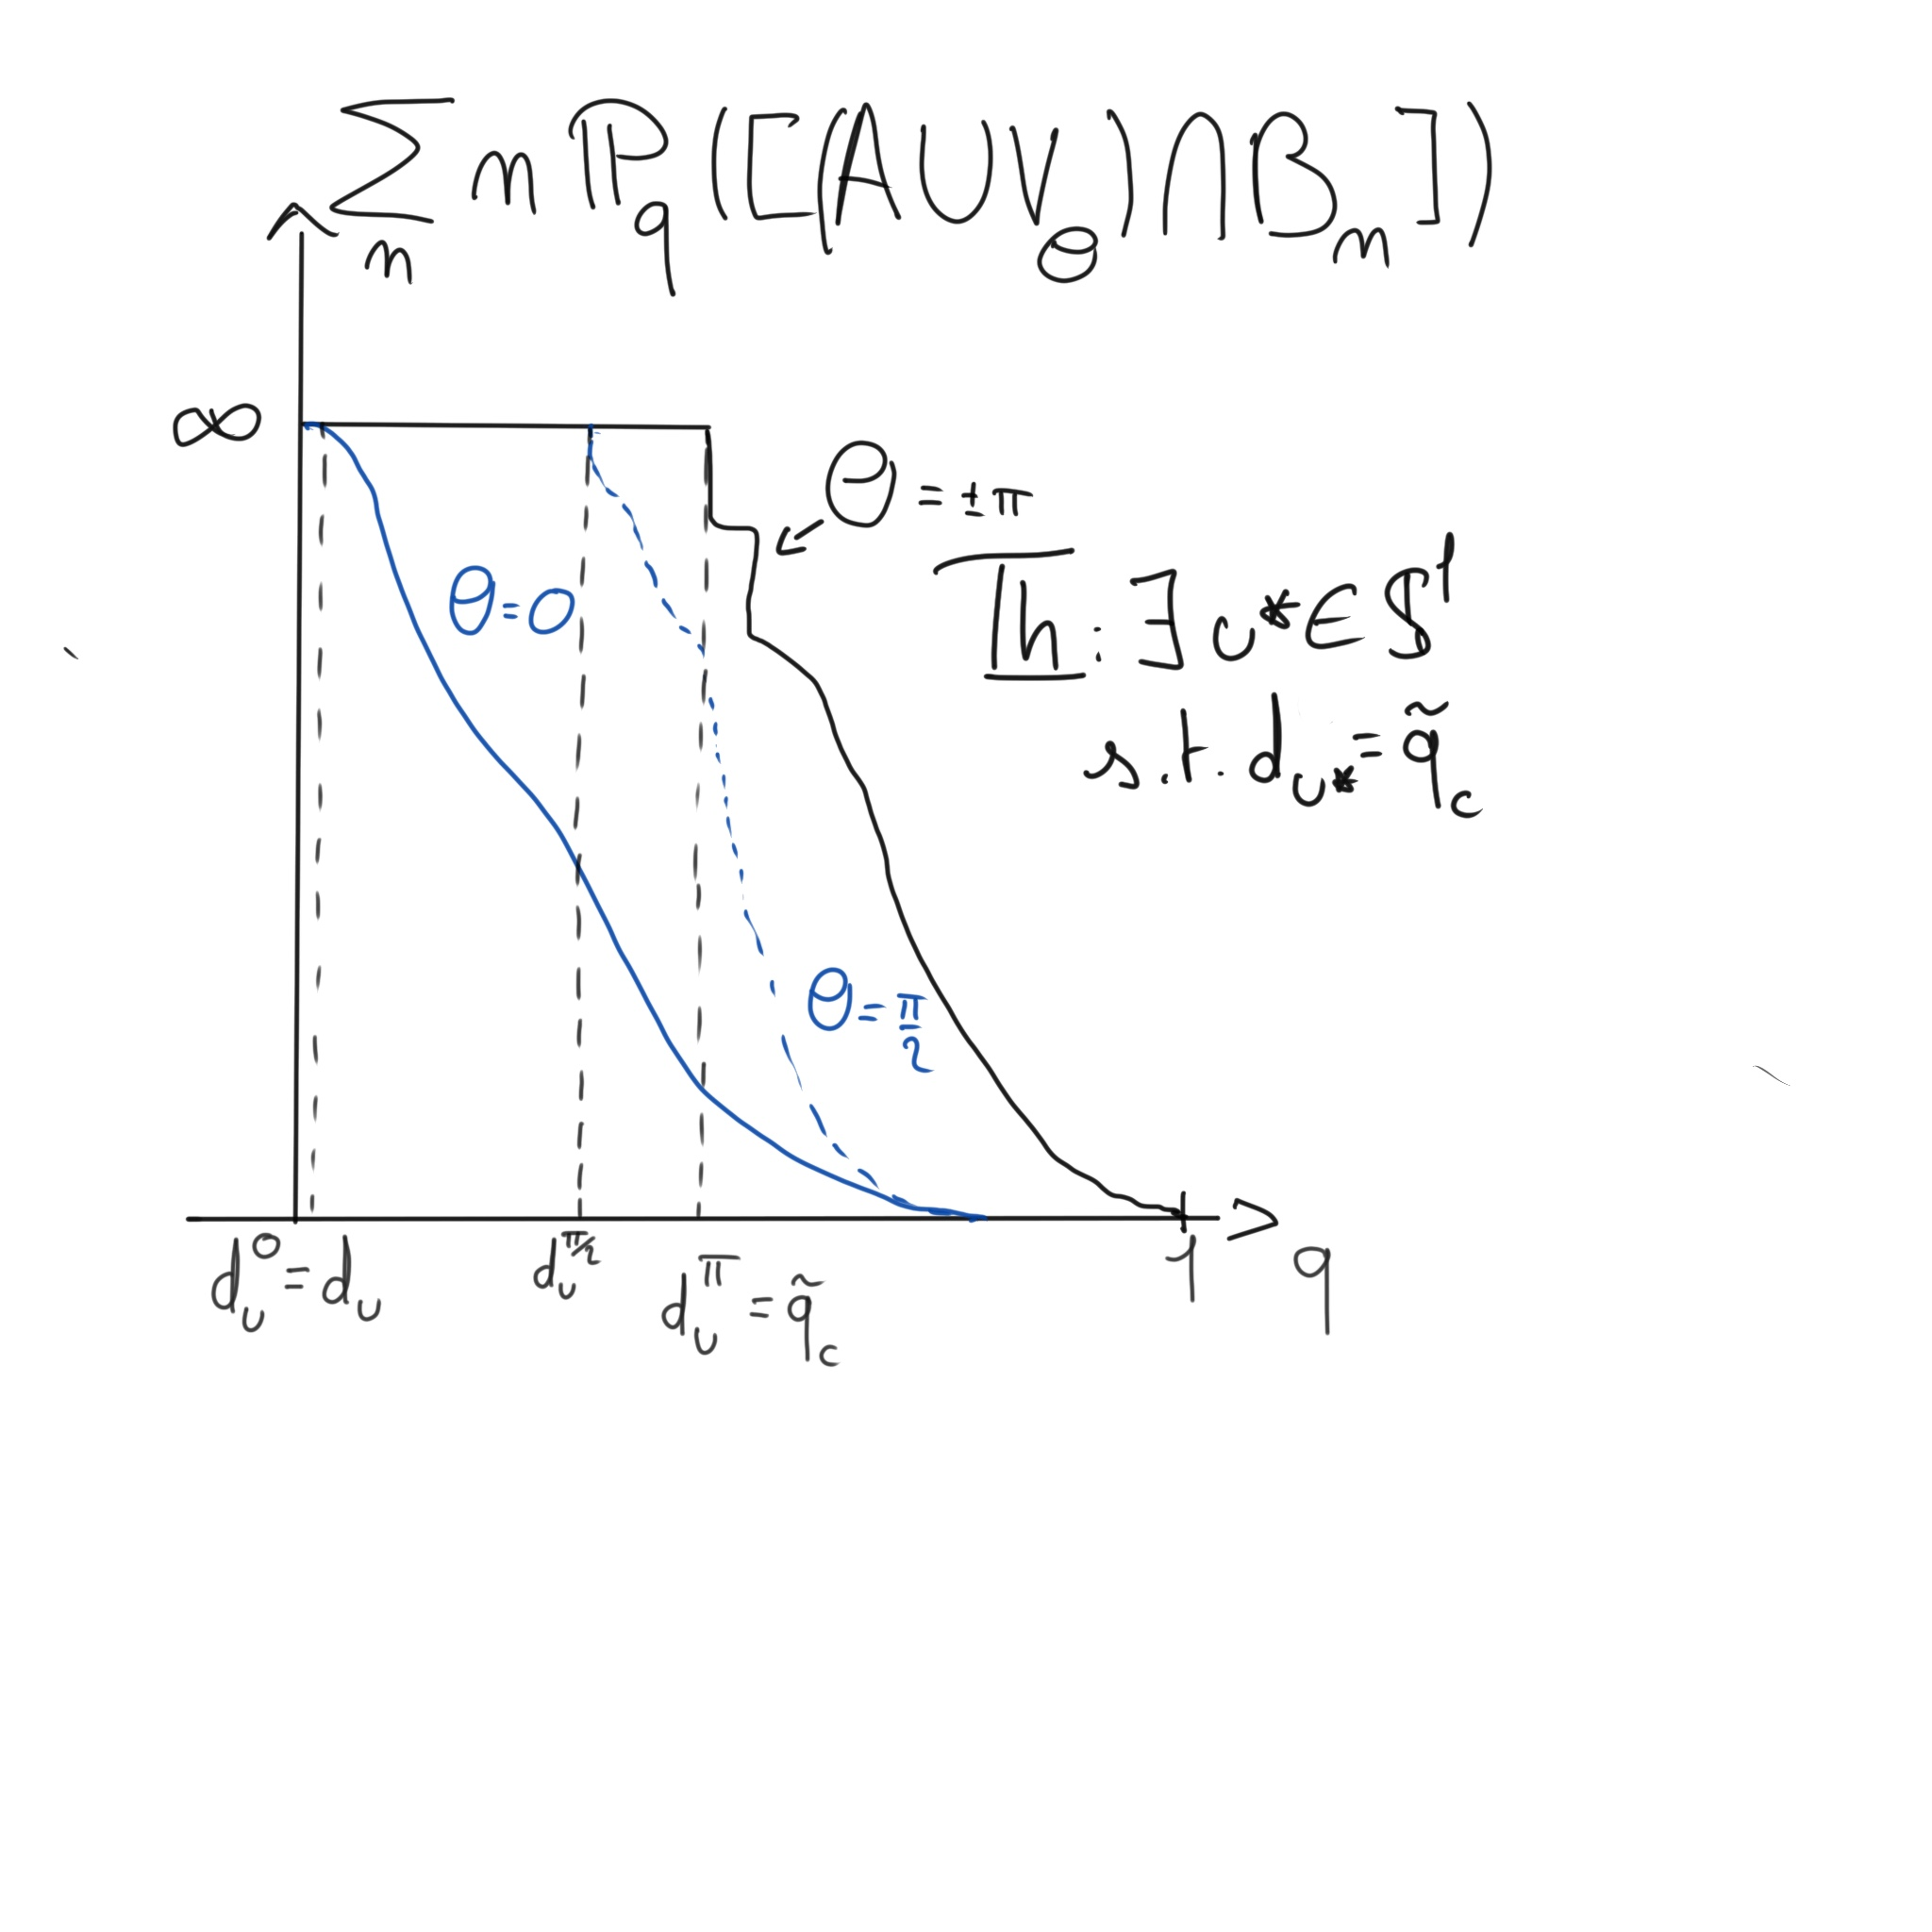
\includegraphics[width=\textwidth]{decay_theta.jpg}
\end{column}
\begin{column}{0.6\textwidth}  
    \begin{center}
     %%%%% this is a minipage, so \textwidth is already adjusted to the size of the column
     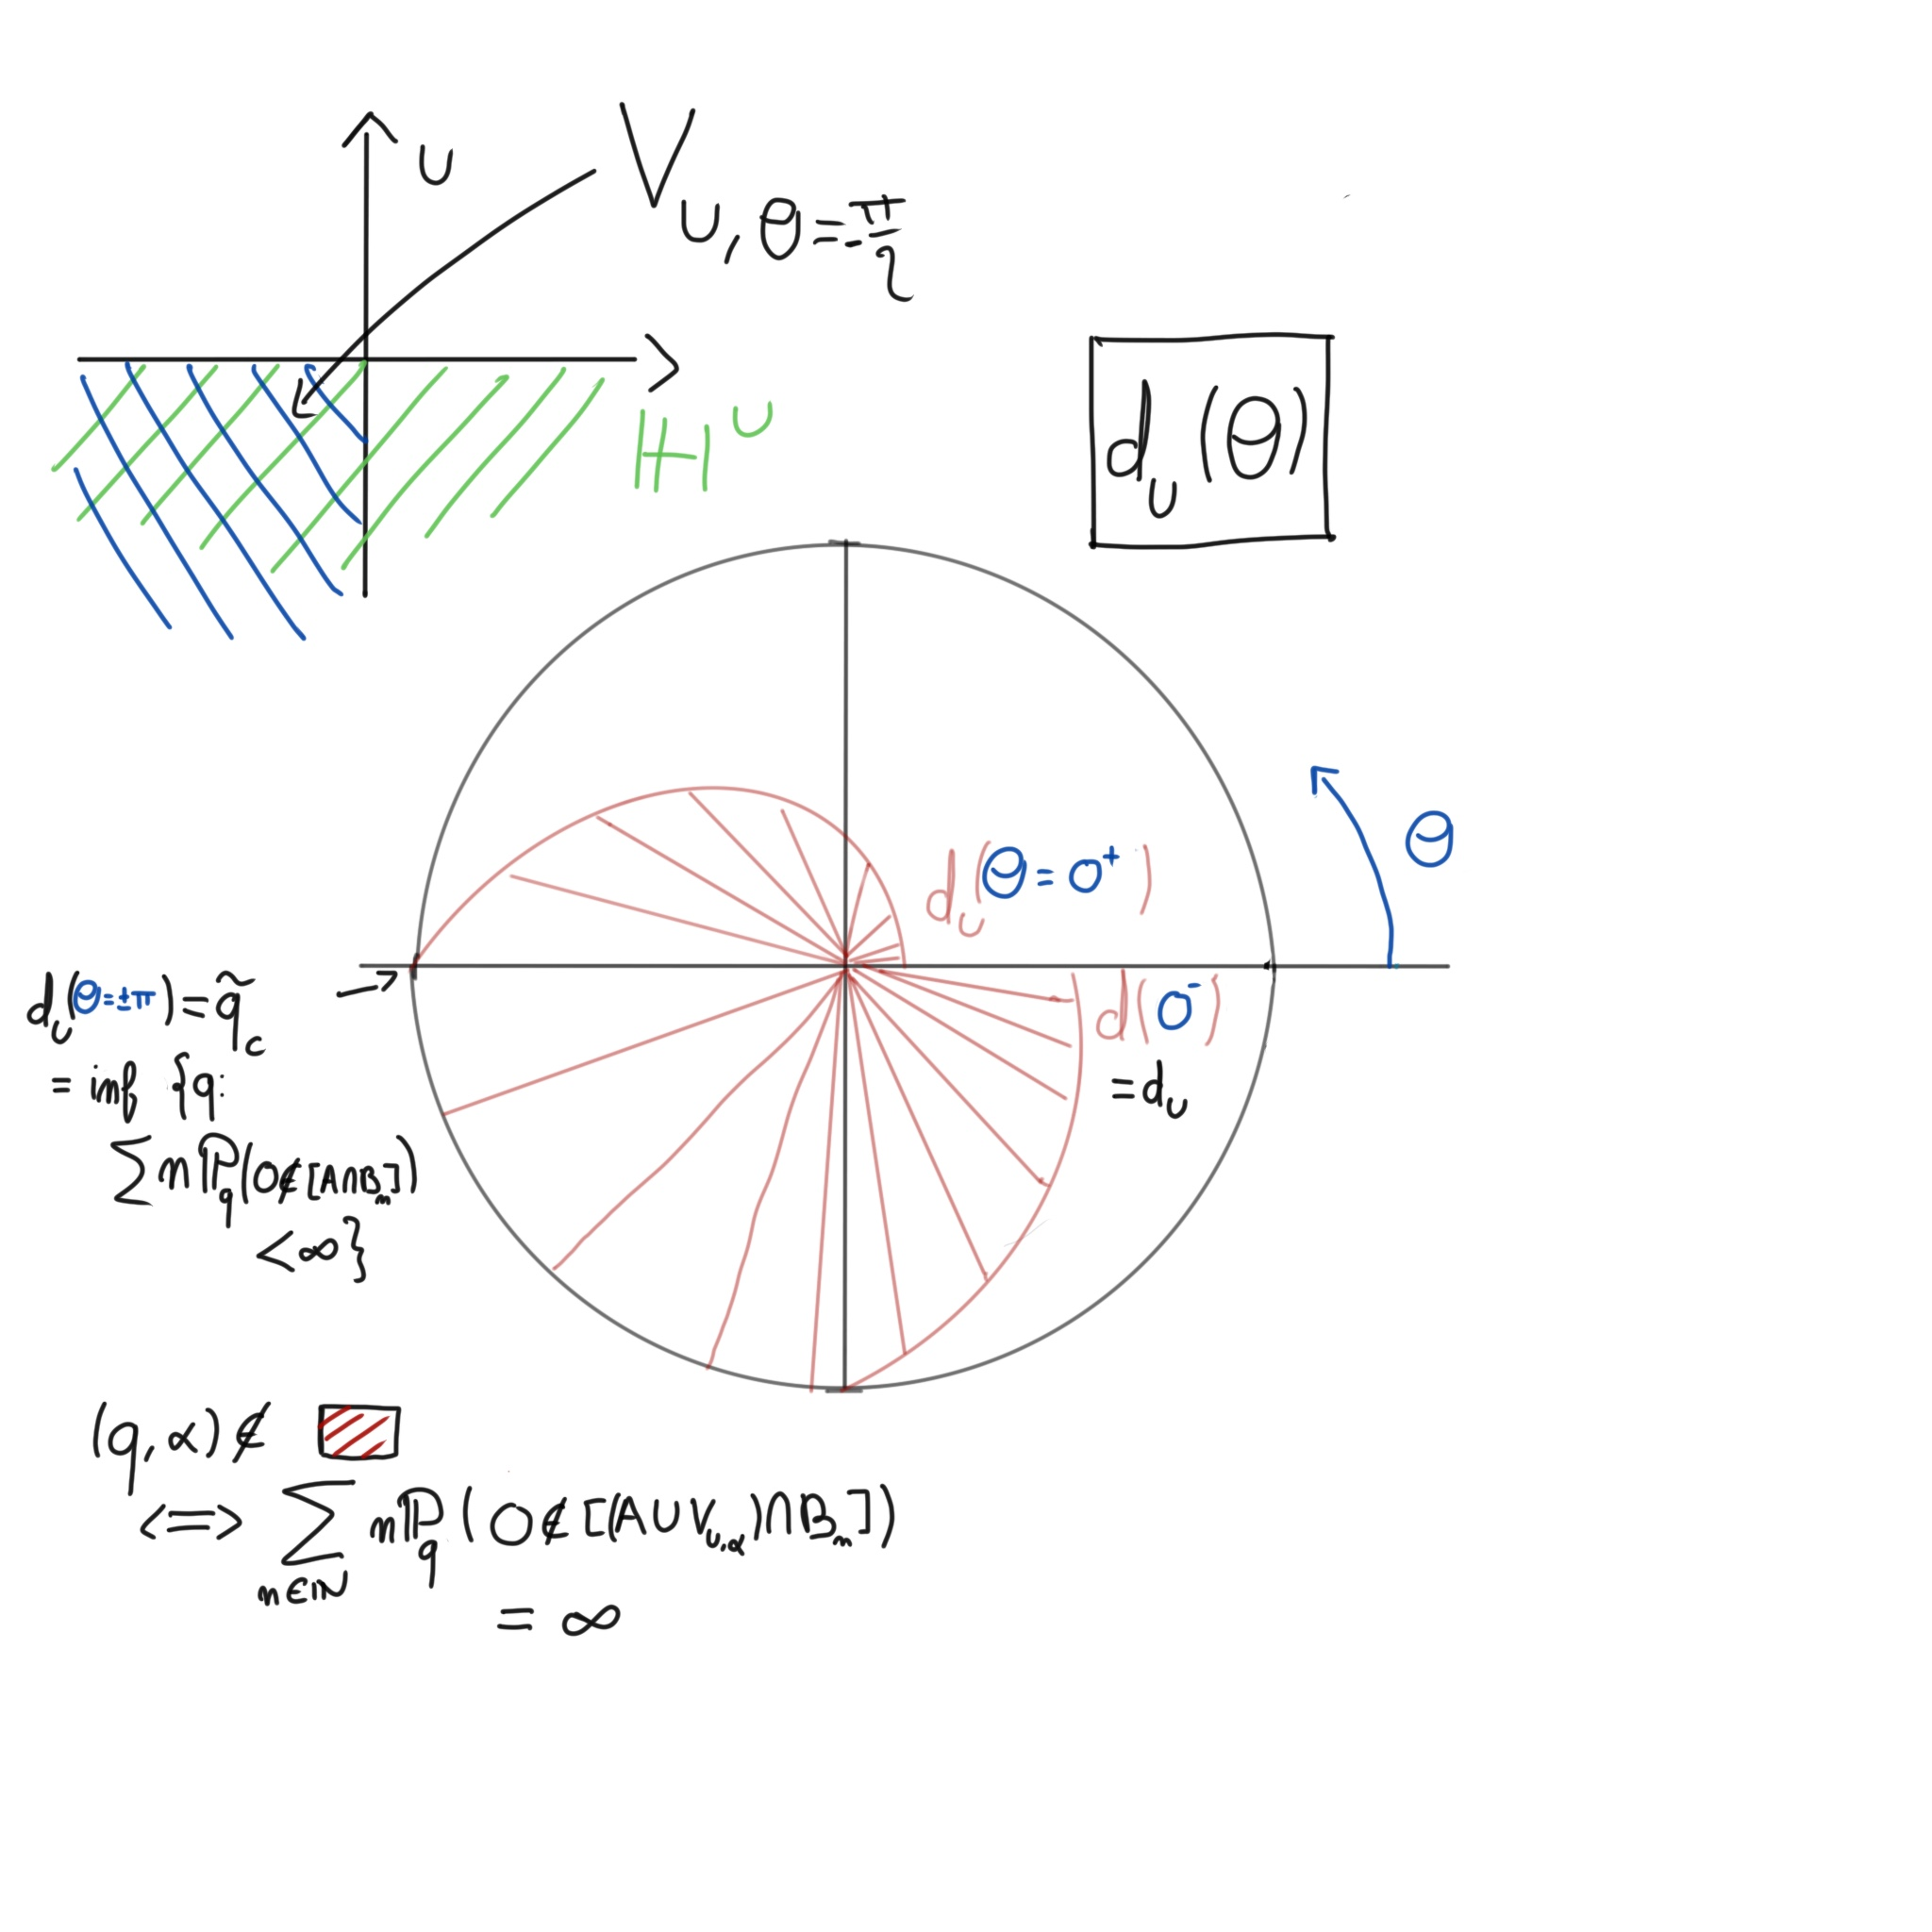
\includegraphics[width=1.1\textwidth]{diag_theta.jpg}
     \end{center}
\end{column}
\end{columns}
\end{frame}

\begin{frame}{Monotonicity}
	Let's denote $E_{u, \theta} = \{0\not\in [(A\cup V_{u, u+\theta})\cap B_n]\}$. Then,
	\begin{equation*}
		E_{u, \pm\pi} = \{ 0 \not\in [A\cap B_n]\} \supset E_{u, \theta}
	\end{equation*}
	which gives that the following holds for any $u$
	\begin{equation*}
		\tilde q_c \geq \sup_\theta \sup_u d_u^\theta \geq \limsup_{\theta\to 0} \sup_u d_u^\theta = \sup_u d_u.
	\end{equation*}
	The theorem states that all those quantities are equal. 
	\begin{block}{Meaning of the theorem}
		The difficulty of the model is as hard as its most difficult direction. In this direction, infecting a half plane doesn't affect the infection of the origin.
	\end{block}
\end{frame}

\begin{frame}{Consequence of monotonicity}
	\begin{center}
    	 	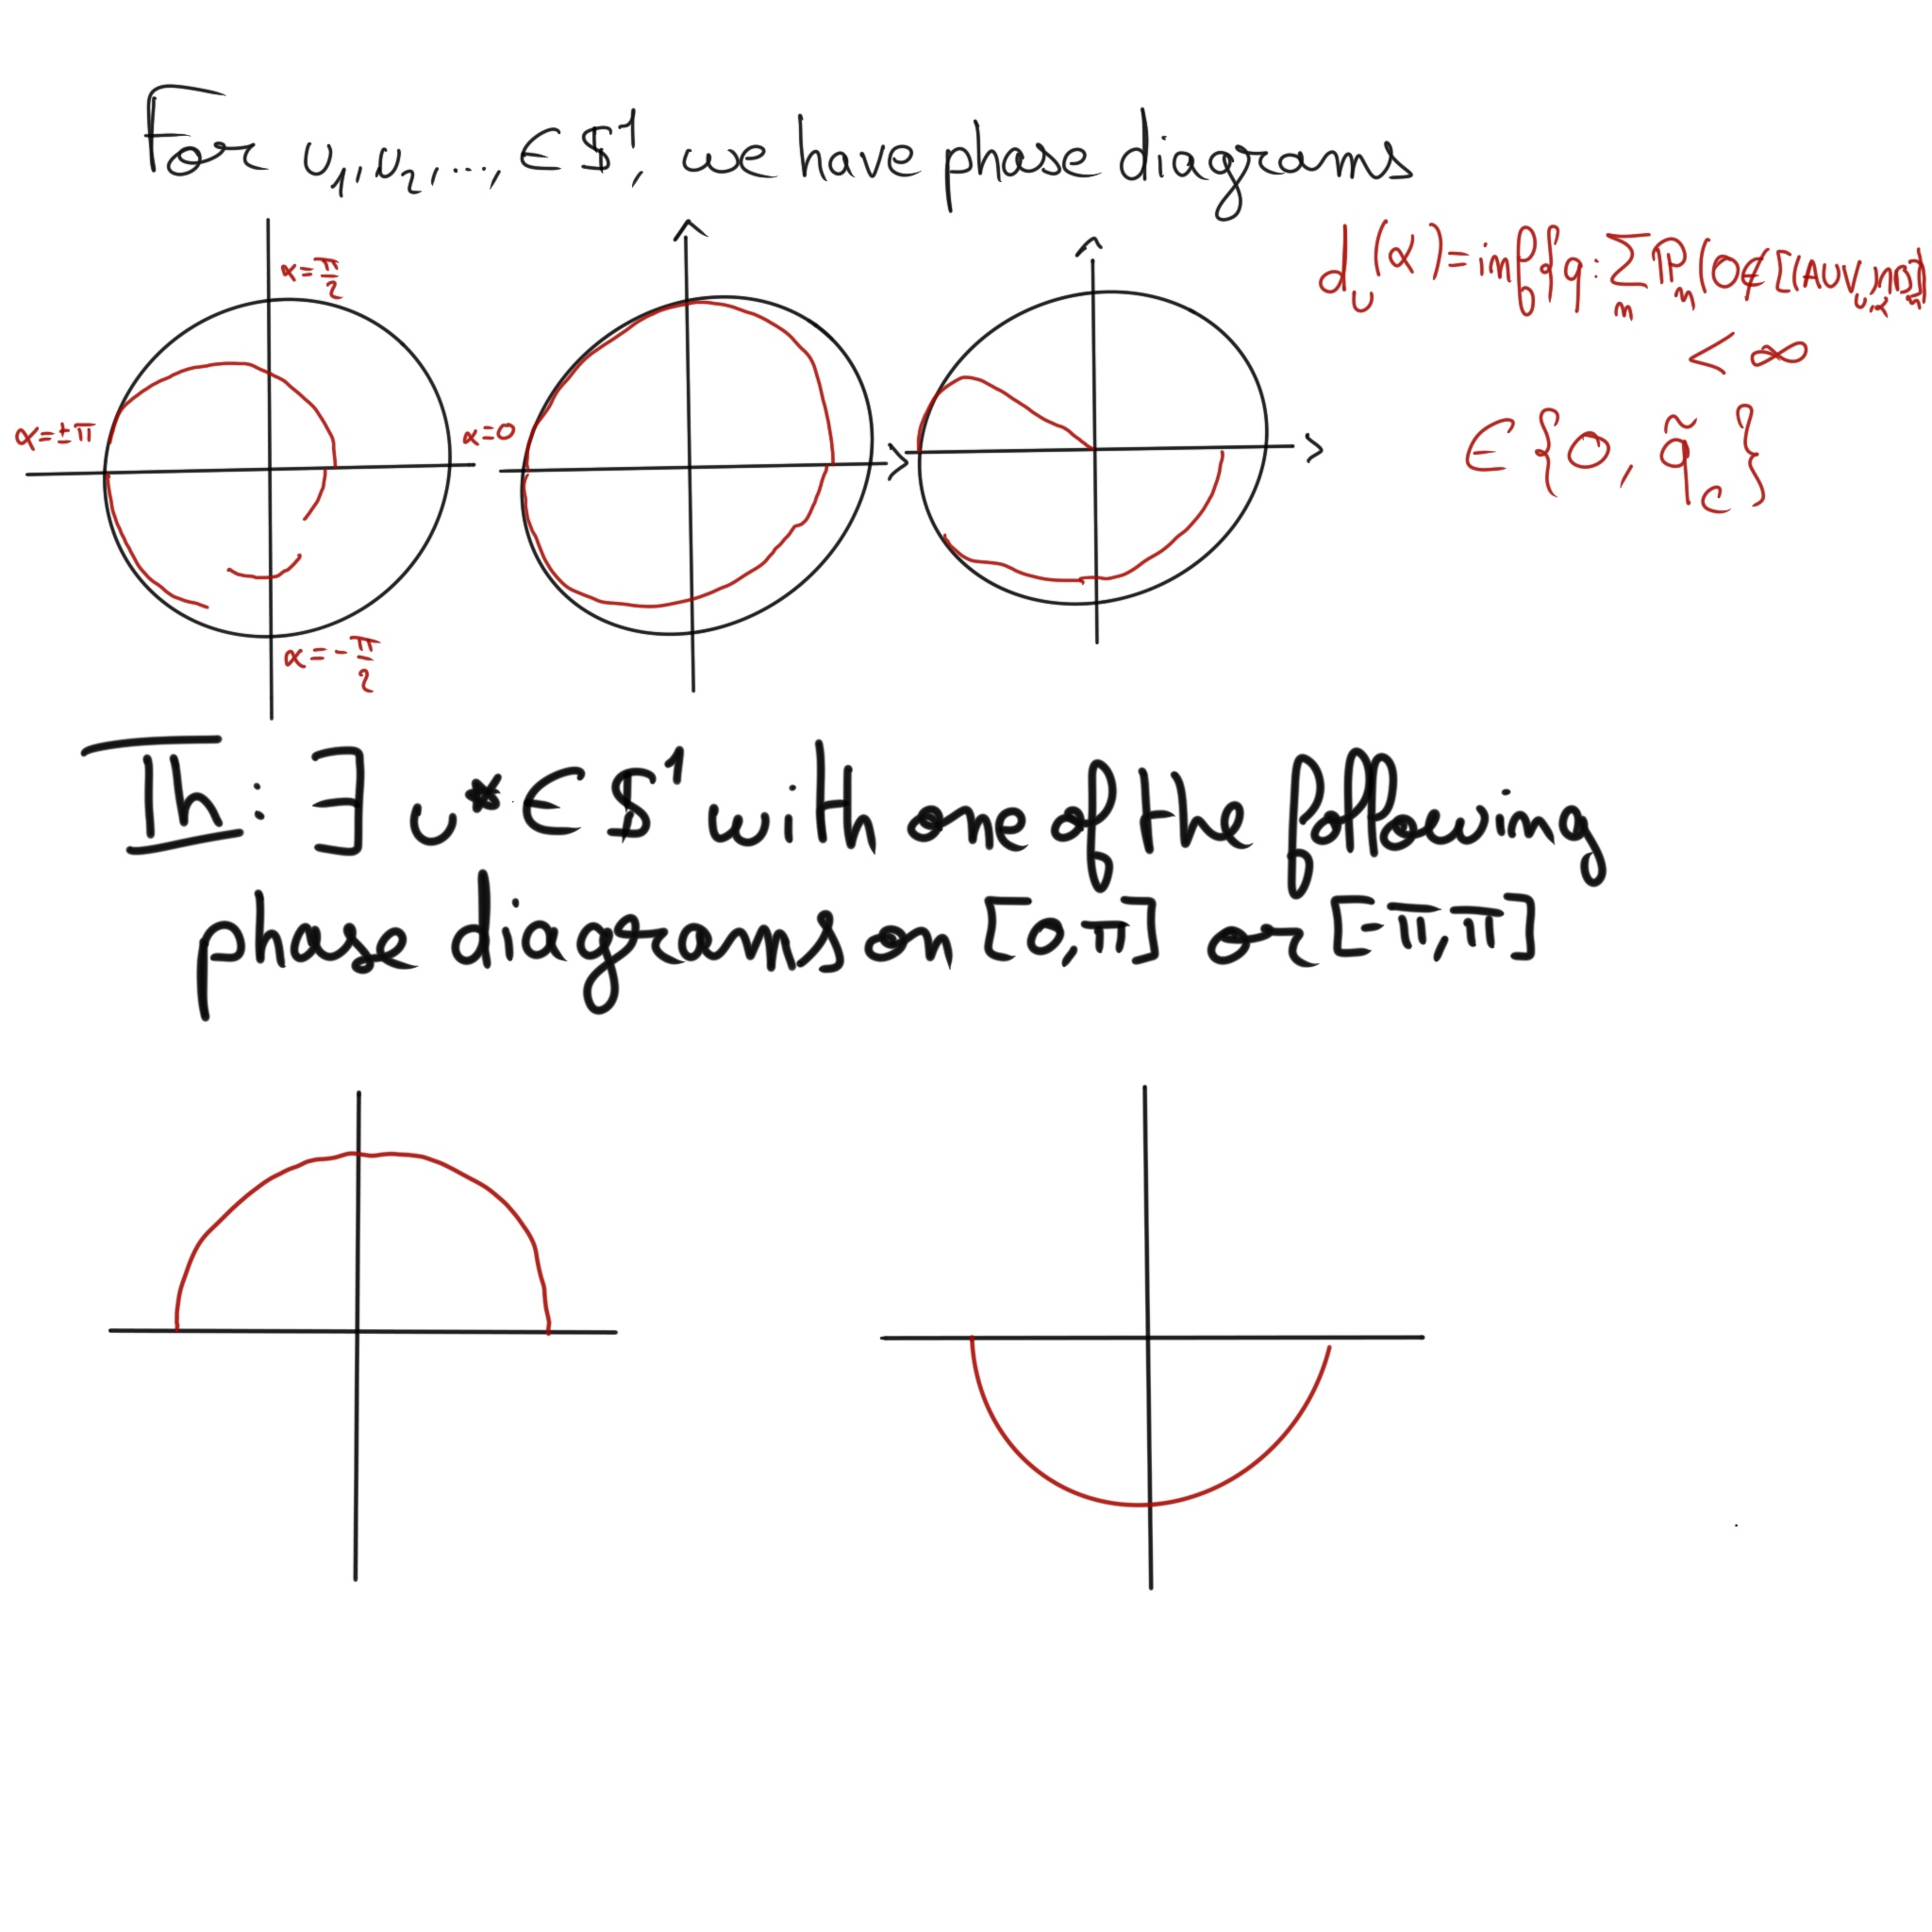
\includegraphics[width=0.9\textwidth]{semi_circ.jpg}
	\end{center}
\end{frame}

\begin{frame}
	\begin{center}
    	 	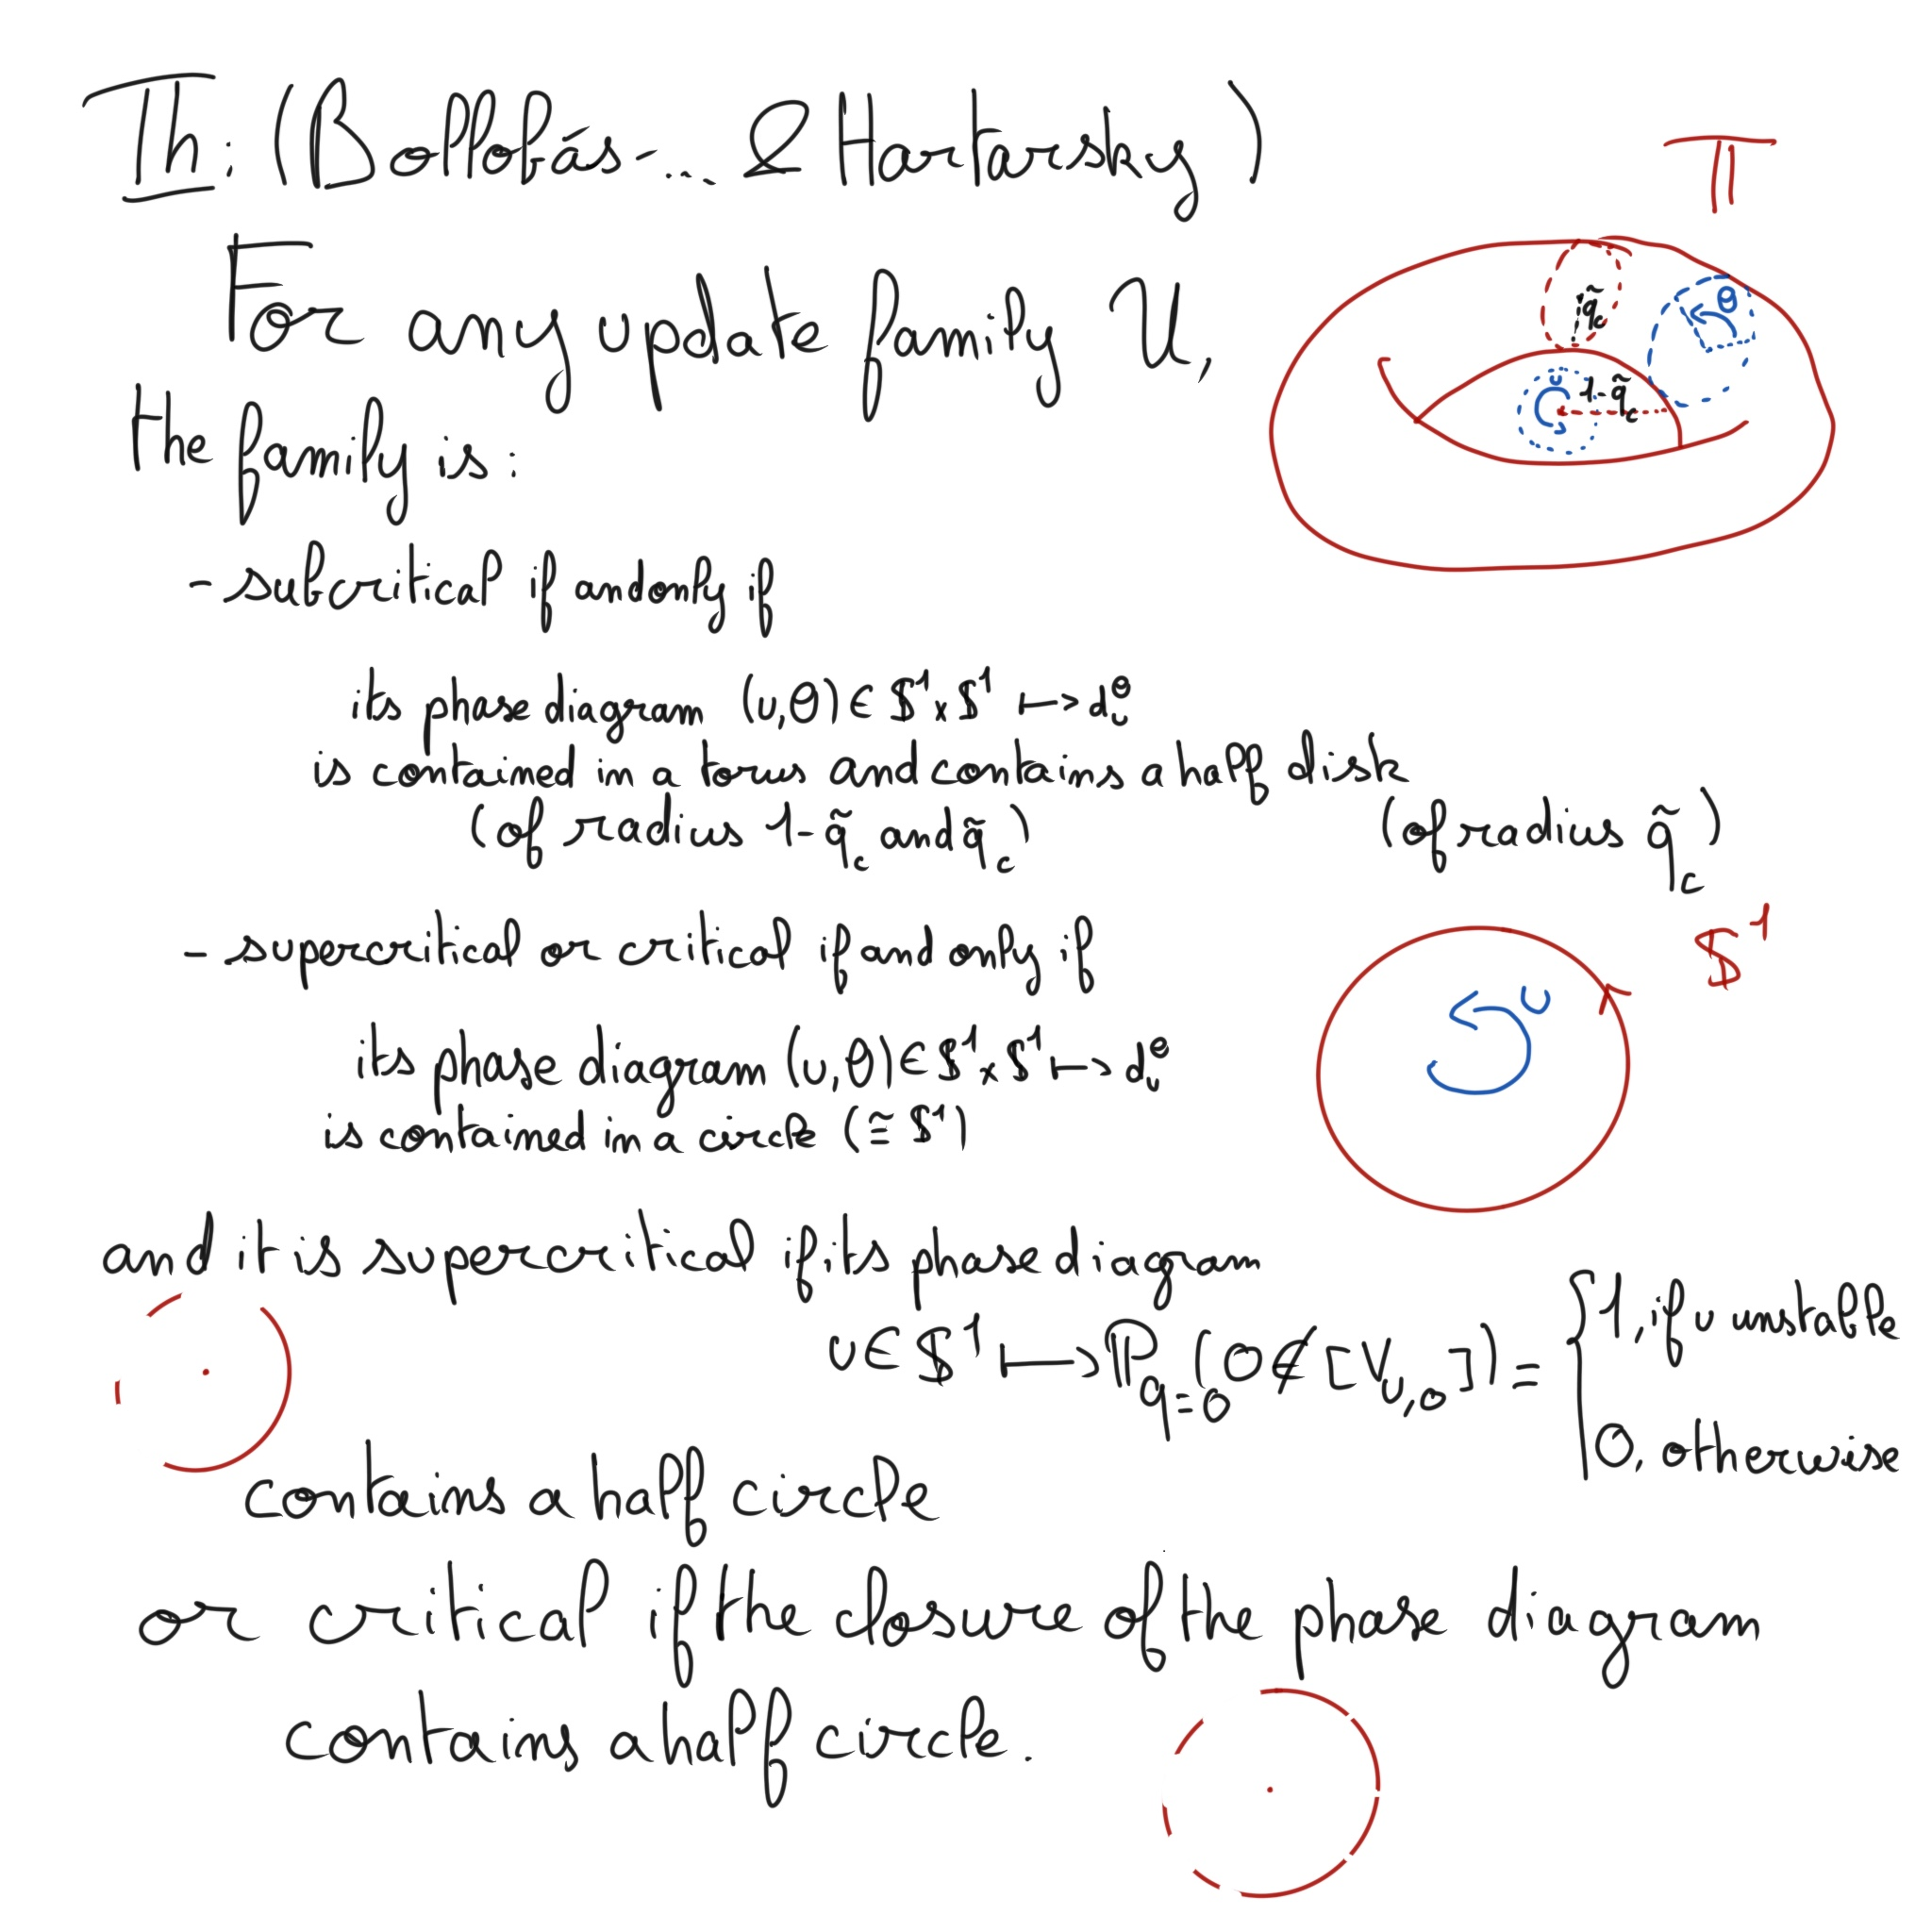
\includegraphics[width=\textwidth]{th_fig.jpg}
	\end{center}
\end{frame}

\begin{frame}{Proving $\sup d_u \geq \tilde q_c$}
	The goal is to show, that for any $q'>\sup d_u$ it holds that
	\begin{equation*}
		\sum_n n \mathbb{P}_{q'}(0\not\in[A\cap B_n]) < \infty.
	\end{equation*}
	The idea is to show that, at $q'$, the origin is infected most of the time.
	\begin{block}{2-step percolation : $q' = \sup d_u + \varepsilon$}
		\begin{enumerate}
			\item Infect sites with probability $\varepsilon$ to find some structures
			\item Infecting new sites with probability $q$ allows structures to grow
		\end{enumerate}
	\end{block}
\end{frame}

\begin{frame}{Some details on the proof}
	\begin{itemize}
		\item The structures that grow are droplets, with sides $(u_i)_{i=1}^n$ depending on $\sup d_u$.
		\item In the second percolation, droplets of size $L$ grow into droplets of size $\geq (1+\delta)L$, for some $\delta > 0$.
		\item The proof can be done in any semi-circle, so we can get $\tilde q_c = \inf_{C\in\mathcal{C}}\sup_{u\in C} d_u$
		\item The proof contains that $\forall q> \sup d_u$, there exists a constant $c(q)>0$ such that
			\begin{equation*}
				\theta_n(q) \leq e^{-c(q)n}
			\end{equation*}
	\end{itemize}
	\begin{center}
    	 	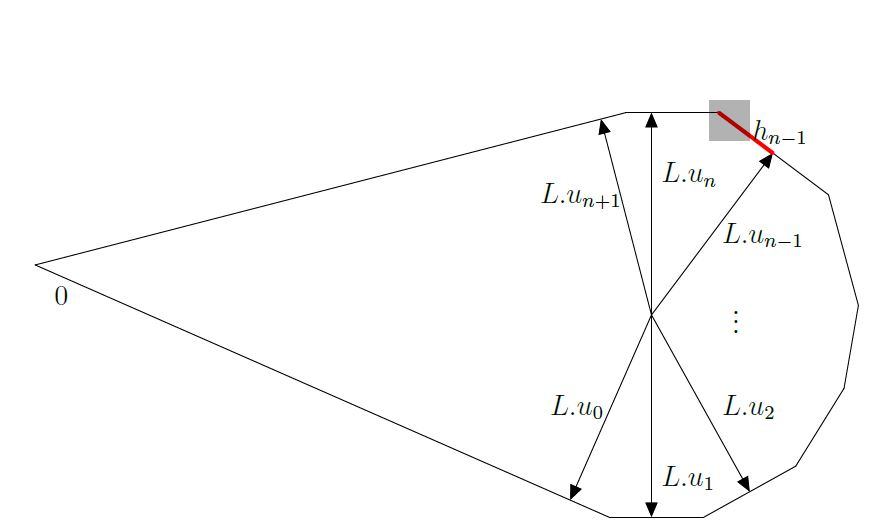
\includegraphics[width=0.5\textwidth]{droplet.jpg}
	\end{center}
\end{frame}

\begin{frame}{Applying the theorem}
	\begin{theorem}
		For any update rules $\mathcal{U}$,
		\begin{equation*}
			q_c \leq \tilde q_c = \sup_{u\in\mathbb{S}^1} d_u = \inf_{C\in\mathcal{C}} \sup_{u\in C} d_u.
		\end{equation*}
		In particular, if $\mathcal{U}$ is not subcritical, then $\tilde q_c = q_c = 0$ 
	\end{theorem}
	So, having knowledge on $u\mapsto d_u$ allows to upper bound $q_c$...
	\begin{block}{Proposition : (It's harder for submodels to infect)}
		For any sub-collection of rules $\mathcal{U}'\subset \mathcal{U}$
		\begin{equation*}
			q_c(\mathcal{U}) \leq \tilde q_c (\mathcal{U}) \leq \inf_C \sup_{u\in C} d_u(\mathcal{U'})
		\end{equation*}
	\end{block}
	... and it is not even necessary to know the critical density for the whole set of rules to get such bounds.
\end{frame}

\begin{frame}{First level bound}
	\begin{block}{$DTBP$ : Directed Triangular Bootstrap Percolation}
		Let $\mathcal{U}' = \{(-1, -1), (0,1)\}$, one of the rules of DTBP, then
		\begin{equation*}
			q_c(DTBP) \leq \tilde q_c(DTBP) \leq \inf_{C\in\mathcal{C}} \sup_{u\in C} d_u(\mathcal{U}').
		\end{equation*}
		Applying a general formula for one rule families (using OP) gives $q_c(DTBP) \leq 0.245...$\footnote{Previous known bound was 0.312}
	\end{block}
	\begin{center}
    	 	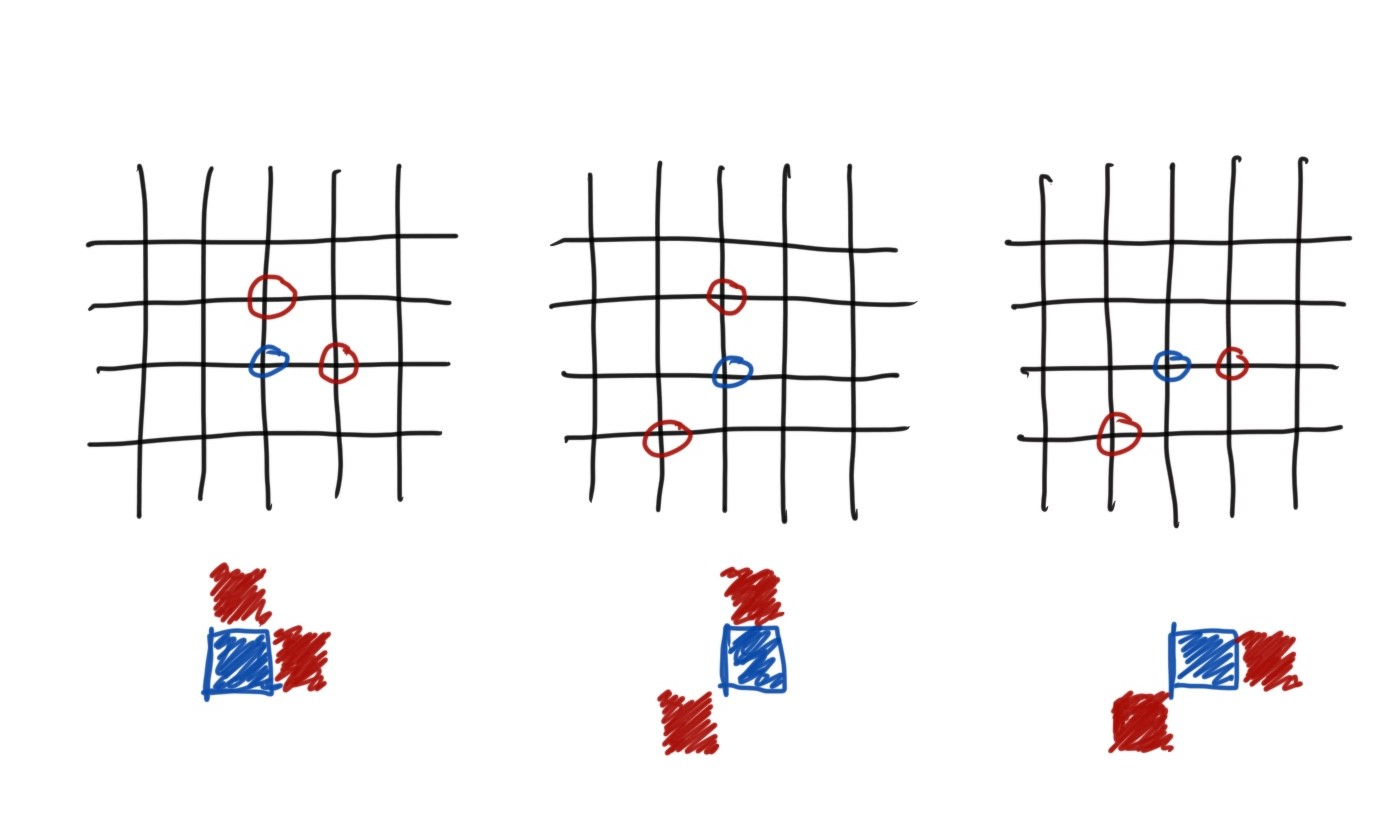
\includegraphics[width=0.5\textwidth]{dtbp.jpg}
	\end{center}
\end{frame}

\begin{frame}{Second level bound}
	However, knowing subfamilies with a single rule is not enough.
	\begin{block}{Spiral}
		For spiral, it is possible to compute $d_u$ for all pairs of rules, such that the difficulty on pairs is the same as the difficulty of some Bidirectional OP :
		\begin{equation*}
			q_c(Spiral) \leq \tilde q_c(Spiral) \leq 1 - p_c^{OP}.
		\end{equation*}
		And the result is tight.
	\end{block}
	\begin{center}
    	 	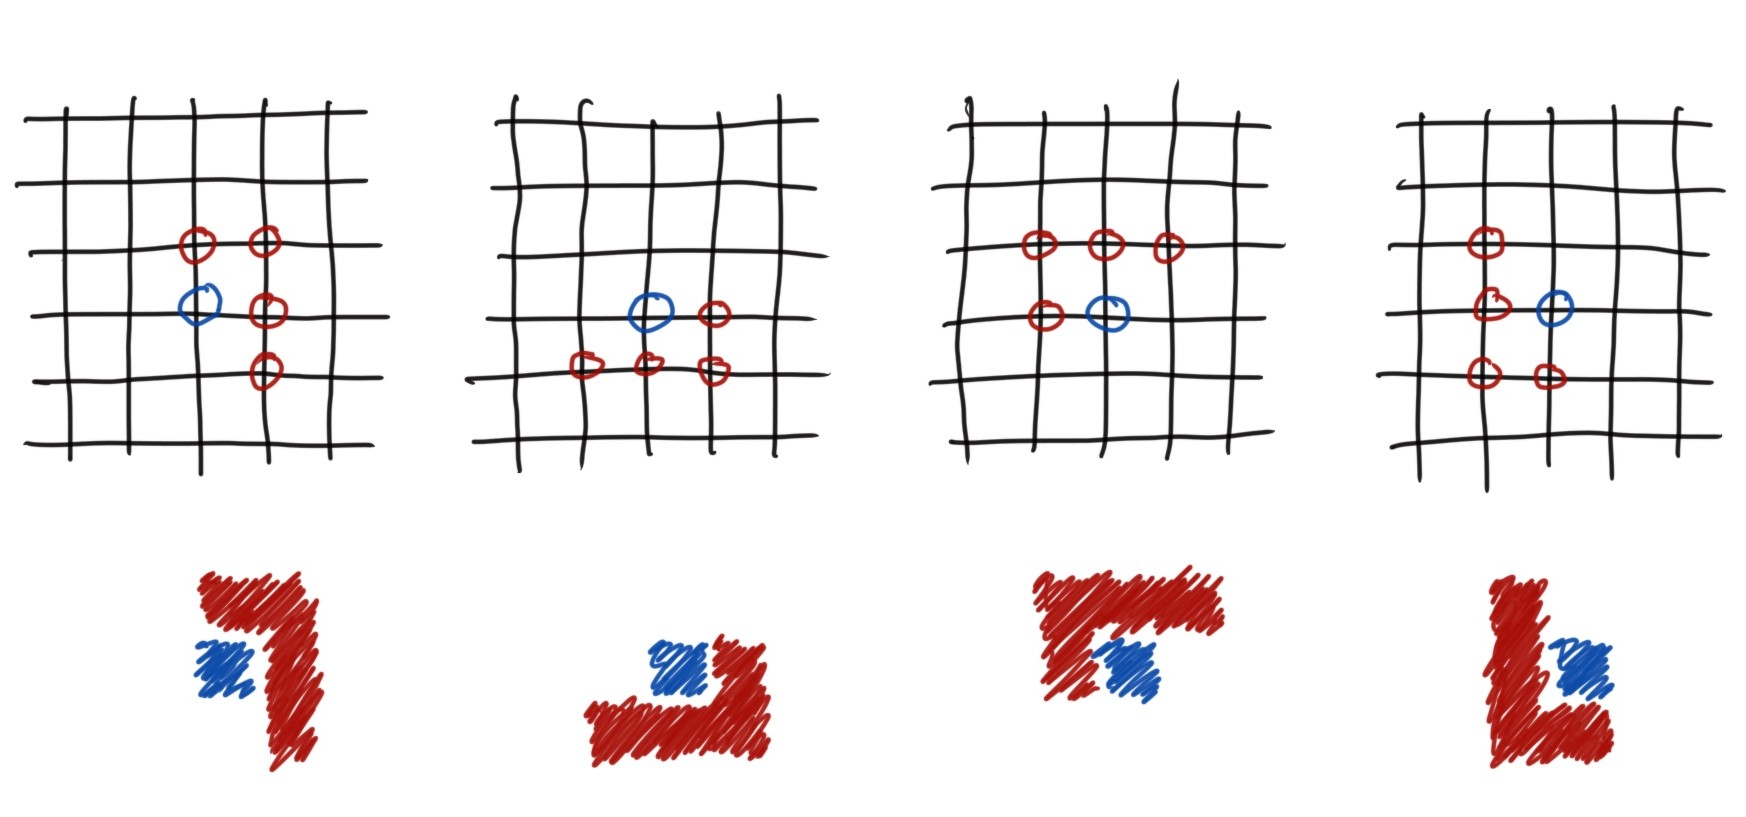
\includegraphics[width=0.5\textwidth]{spiral.jpg}
	\end{center}
\end{frame}
